\subsubsection{NodeJS}
\subsubsubsection{NodeJS là gì}

\begin{center}
  \captionsetup{type=figure}
  \includesvg[width=10cm]{img/nodejs.svg}
  \captionof{figure}{NodeJS}
\end{center}


NodeJS là một mã nguồn được xây dựng dựa trên nền tảng Javascript V8 Engine, nó được sử dụng để xây dựng các ứng dụng web như các trang video clip, các forum và đặc biệt là trang mạng xã hội phạm vi hẹp. NodeJS là một mã nguồn mở được sử dụng rộng bởi hàng ngàn lập trình viên trên toàn thế giới. NodeJS có thể chạy trên nhiều nền tảng hệ điều hành khác nhau từ Windows cho tới Linux, OSX nên đó cũng là một lợi thế. NodeJS cung cấp các thư viện phong phú ở dạng Javascript module khác nhau giúp đơn giản hóa việc lập trình và giảm thời gian ở mức thấp nhất.

\subsubsubsection{Đặc điểm của NodeJS}

\begin{itemize}
  \item \textbf{Realtime:} Đây là tính năng quan trọng nhất của NodeJS. Realtime ở đây chính là xử lý giao tiếp từ client tới máy chủ theo thời gian thực. Giống như khi bạn lướt Facebook thì mỗi khi bạn comment hay like một topic nào đó thì ngay lập tức chủ topic và những người đã comment trên đó sẽ nhận được thông báo là bạn đã comment.
  \item \textbf{Không đồng bộ:} Tất cả các API của NodeJS đều không đồng bộ (none-blocking), nó chủ yếu dựa trên nền của NodeJS Server và chờ đợi Server trả dữ liệu về. Việc di chuyển máy chủ đến các API tiếp theo sau khi gọi và cơ chế thông báo các sự kiện của Node.js giúp máy chủ để có được một phản ứng từ các cuộc gọi API trước (Realtime).
  \item \textbf{Chạy rất nhanh:} NodeJ được xây dựng dựa vào nền tảng V8 Javascript Engine nên việc thực thi chương trình rất nhanh.
  \item \textbf{Đơn luồng nhưng khả năng mở rộng cao:} Node.js sử dụng một mô hình luồng duy nhất với sự kiện lặp. cơ chế tổ chức sự kiện giúp các máy chủ để đáp ứng một cách không ngăn chặn và làm cho máy chủ cao khả năng mở rộng như trái ngược với các máy chủ truyền thống mà tạo đề hạn chế để xử lý yêu cầu. Node.js sử dụng một chương trình đơn luồng và các chương trình tương tự có thể cung cấp dịch vụ cho một số lượng lớn hơn nhiều so với yêu cầu máy chủ truyền thống như Apache HTTP Server.
  \item \textbf{Không đệm:} NodeJS không đệm bất kì một dữ liệu nào và các ứng dụng này chủ yếu là đầu ra dữ liệu.
  \item \textbf{Có giấy phép:} NodeJS đã được cấp giấy phép bởi MIT License.
\end{itemize}

\subsubsubsection{NodeJs được sử dụng ở đâu}
\begin{itemize}
  \item \textbf{Websocket server:} Các máy chủ web socket như là Online Chat, Game Server…
  \item \textbf{Fast File Upload Client:} Là các chương trình upload file tốc độ cao.
  \item \textbf{Ad Server:} Các máy chủ quảng cáo.
  \item \textbf{Cloud Services:} Các dịch vụ đám mây.
  \item \textbf{RESTful API:} Đây là những ứng dụng mà được sử dụng cho các ứng dụng khác thông qua API.
  \item \textbf{Any Real-time Data Application:} Bất kỳ một ứng dụng nào có yêu cầu về tốc độ thời gian thực. Micro Services: Ý tưởng của micro services là chia nhỏ một ứng dụng lớn thành các dịch vụ nhỏ và kết nối chúng lại với nhau. Nodejs có thể làm tốt điều này.
\end{itemize}

\subsubsubsection{Thế mạnh của NodeJS}
\begin{itemize}
  \item Cú pháp ngắn gọn, dễ nhớ. Đặc biệt dễ học với những ai đã từng làm việc với nhiều với Javascript, Jquery.
  \item Xử lý không đồng bộ tốt: ví dụ khi upload file, chương trình không chờ việc upload xong mới xử lý việc tiếp theo. Nghĩa là trong khi xử lý upload file chương trình vẫn tiếp tục xử lý các công việc mới.
  \item Khả năng xử lý song song tuyệt vời: NodeJs sẽ tận dụng tối đa Unix để hoạt động. Tức là NodeJs có thể xử lý hàng nghìn process và trả ra 1 luồng khiến cho hiệu xuất hoạt động đạt mức tối đa nhất.
  \item Có nhiều packages hỗ trợ để tạo nhiều chức năng cho site, các packages được cài đặt bằng câu lệnh giống như cài đặt gem trong ruby on rails.
  \item Hỗ trợ nhiều template engine để render view.
  \item Có nhiều framework. Được sử dụng phổ biến nhất là : ExpressJs, SailsJS.
  \item Khả năng sử dụng lại code: dễ dàng tạo ra các module, helper, library để sử dụng ở nhiều nơi.
  \item Hỗ trợ security tốt. NodeJs mặc định hỗ trợ chống tấn công Cross-site script.
\end{itemize}

\subsubsubsection{ExpressJS}
\begin{center}
  \captionsetup{type=figure}
  
\includegraphics[width=15cm]{img/expressjs.png}
  \captionof{figure}{Express JS}
\end{center}

Express.js được xây dựng bởi TJ Holowaychuk, một thành viên trong team Node đã tạo ra Node.js. Cũng chính vì vậy mà đây là một trong những framework quan trọng nhất của Node.js. Expressjs cung cấp các hàm HTTP và midleware để tạo ra API đơn giản và dễ sử dụng. Express.js là một framework tối giản để xây dựng một loạt các ứng dụng web và di động cũng như các giao diện lập trình ứng dụng (API). Được ủng hộ bởi một cộng đồng lớn, framework này luôn được cập nhật liên tục và cải thiện tất cả những tính năng cốt lõi. Express.js cung cấp nhiều tính năng khác nhau như đơn giản hóa nhiều định tuyến, tích hợp cơ sở dữ liệu … và nhờ đó được dùng cho những ứng dụng phổ biến trên các trang web như MySpace, Geekli.st, Klout, Segment.io và Yummly.

ExpressJS được phát hành theo giấy phép mã nguồn mở, có cộng đồng hỗ trợ lớn, được phép sử dụng cho ứng dụng có mục đích thương mại.

Cấu trúc thư mục dự án khi sử dụng ExpressJS được chia là 3 phần: routes, Views và Public. ExpressJS xây dựng ứng dụng web theo đúng mô hình MVC (Model - View - Controller).

\textbf{Một số chức năng chính của ExpressJS:}
\begin{itemize}
  \item Hỗ trợ middleware để trả về các HTTP request.
  \item Định nghĩa route dựa trên các action của HTTP (CRUD).
  \item Cho phép trả về các trang html sử dụng các template engine (jade, pug…).
\end{itemize}

\subsubsubsection{Middleware trong ExpressJS:}

Middleware trong ngành công nghệ phần mềm được định nghĩa là một phần mềm có nhiệm vụ làm cầu nối (bridge), cung cấp các dịch vụ từ phía hệ điều hành đến các ứng dụng, giúp các ứng dụng có thể tương tác với các thành phần được hệ điều hành cho phép. Middleware được coi là chất kết dính dữa các phần mềm với nhau.

\textbf{Middleware trong Web:} 

Với tư tưởng chung là cầu nối giữa tương tác của người dùng và phần nhân của hệ thống, trong lập trình Web, Middleware sẽ đóng vai trò trung gian giữa request/response (tương tác với người dùng) và các xử lý logic bên trong web server.Do đó, Middleware trong các Framework lập tình Web (Django, Rails, ExpressJS), sẽ là các hàm được dùng để tiền xử lý, lọc các request trước khi đưa vào xử lý logic hoặc điều chỉnh các response trước khi gửi về cho người dùng.

\begin{center}
  \captionsetup{type=figure}
  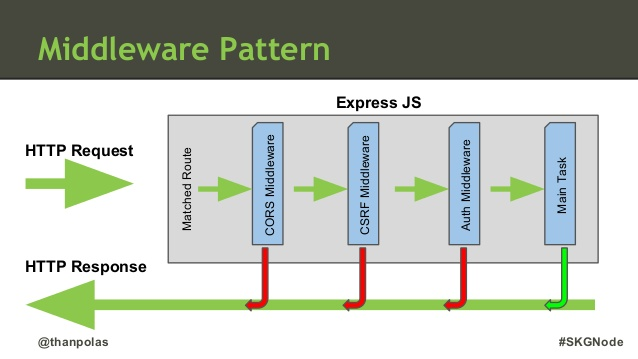
\includegraphics[width=15cm]{img/expressjsmiddleware.jpg}
  \captionof{figure}{Express JS}
\end{center}

Hình trên mô tả 3 middleware có trong ExpressJS. Một request khi gửi đến Express sẽ được xử lý qua 5 bước như sau :
\begin{itemize}
  \item Tìm Route tương ứng với request.
  \item Dùng CORS Middleware để kiểm tra cross-origin Resource sharing của request.
  \item Dùng CRSF Middleware để xác thực CSRF của request, chống fake request.
  \item Dùng Auth Middleware để xác thực request có được truy cập hay không.
  \item Xử lý công việc được yêu cầu bởi request (Main Task).
\end{itemize}

Bất kỳ bước nào trong các bước 2, 3, 4 nếu xảy ra lỗi sẽ trả về response thông báo cho người dùng, có thể là lỗi CORS, lỗi CSRF hay lỗi auth tùy thuộc vào request bị dừng ở bước nào.
\textbf{Middleware trong ExpressJS:} 

ExpressJS khi hoạt động, về cơ bản sẽ là một loạt các hàm Middleware được thực hiện liên tiếp nhau. Sau khi đã thiết lập, các request từ phía người dùng khi gửi lên ExpressJS sẽ thực hiện lần lượt qua các hàm Middleware cho đến khi trả về response cho người dùng. Các hàm này sẽ được quyền truy cập đến các đối tượng đại diện cho Request - req, Response - res, hàm Middleware tiếp theo - next, và đối tượng lỗi - err nếu cần thiết.

Một hàm Middleware sau khi hoạt động xong, nếu chưa phải là cuối cùng trong chuỗi các hàm cần thực hiện, sẽ cần gọi lệnh next() để chuyển sang hàm tiếp theo, bằng không xử lý sẽ bị treo tại hàm đó.

Các chức năng mà middleware có thể thực hiện trong ExpressJS sẽ bao gồm :
\begin{itemize}
  \item Thực hiện bất cứ đoạn code nào.
  \item Thay đổi các đối tượng request và response.
  \item Kết thúc một quá trình request-response.
  \item Gọi hàm middleware tiếp theo trong stack.
\end{itemize}

Trong Express, có 5 kiểu middleware có thể sử dụng :
\begin{itemize}
  \item Application-level middleware (middleware cấp ứng dụng).
  \item Router-level middleware (middlware cấp điều hướng - router).
  \item Error-handling middleware (middleware xử lý lỗi).
  \item Built-in middleware (middleware sẵn có).
  \item Third-party middleware (middleware của bên thứ ba).
\end{itemize}